%!TEX root = ../thesis.tex

\section{Evaluating User-Driven Co-Evolution}
\label{sec:exemplar_user-driven_co-evo}
Several real-world MDE projects in which user-driven co-evolution has been observed were reported in Chapter~\ref{Analysis}, and Chapters~\ref{LiteratureReview} and~\ref{Analysis} highlighted that no tool support for user-driven co-evolution has yet been reported in the literature. To address this, Chapter~\ref{Implementation} proposed two structures to support user-driven co-evolution, a metamodel-independent syntax (Section~\ref{sec:mmi_syntax}) and a textual modelling notation (Section~\ref{sec:notation}). This section explores the extent to which the two structures increase the productivity of user-driven co-evolution, supporting the research hypothesis which stated that \emph{integrating dedicated structures and processes with contemporary MDE environments is beneficial in terms of increased productivity}.

To explore the hypothesis, several approaches to evaluation could be used. The metamodel-independent syntax and textual modelling notation are freely available as part of Epsilon, a component of the Eclipse Modeling Project, so the productivity benefits of the structures could have been explored by gathering and analysing the opinion of users. However, this approach was discounted because drawing meaningful conclusions would have needed understanding of each user's domain, context and background. Evaluation could have been performed with a comprehensive user study that measured the time taken for developers to perform model migration with and without the dedicated structures for user-driven co-evolution. However, locating developers and co-evolution examples was not possible in the available time. Instead, evaluation was conducted by comparing two approaches to user-driven co-evolution using an example from a real-world MDE project. The first approach uses only the tools available in the Eclipse Modeling Framework (EMF); while the second approach uses EMF together with the metamodel-independent syntax and textual modelling notation introduced in Chapter~\ref{Implementation}.

Section~\ref{subsec:challenges_for_performing_user-driven_co-evo} summarises Section~\ref{subsec:user-driven_co-evolution}, which described the challenges to productivity faced by developers while performing user-driven co-evolution with EMF. Section~\ref{subsec:user-driven_co-evolution_example} introduces the example of user-driven co-evolution used to perform the evaluation. In Sections~\ref{subsec:user-driven_co-evolution_with_emf} and~\ref{subsec:user-driven_co-evolution_with_dedicated_structures}, the two approaches to user-driven co-evolution are demonstrated. The section concludes by comparing the two approaches and highlighting ways in which the metamodel-independent syntax and textual modelling notation increase developer productivity in the context of user-driven co-evolution.

\subsection{Challenges for Performing User-Driven Co-Evolution}
\label{subsec:challenges_for_performing_user-driven_co-evo}
Two productivity challenges for performing user-driven co-evolution in contemporary MDE environments were identified in Section~\ref{subsec:user-driven_co-evolution}. Firstly, model storage representations are not optimised for use by humans, and so user-driven co-evolution -- which typically involves changing models by hand -- is made error-prone and time consuming. Secondly, the multi-pass parsers used to load models in contemporary MDE environments make user-driven co-evolution an iterative process, because not all conformance errors are reported in the first pass. The identification of these productivity challenges led to the derivation of the following research requirement in Section~\ref{sec:requirements_identification}: \emph{This thesis must demonstrate a user-driven co-evolution process that enables the editing of non-conformant models without directly manipulating the underlying storage representation and provides a conformance report for the original model and evolved metamodel.}

Two of the structures presented in Chapter~\ref{Implementation} provide the foundation for fulfilling the above research requirement. The first, a metamodel-independent syntax, facilitates the conformance checking of a model against any metamodel. The second structure, the textual modelling notation \emph{Epsilon HUTN}, allows models to be managed in a format that is reputedly easier for humans to use than XMI, the canonical model storage format \cite{hutn}.

To fulfil the above research requirement, this section applies the me\-ta\-mo\-del-ind\-ep\-en\-de\-nt syntax and the textual modelling notation to demonstrate that user-driven co-evolution can be performed without encountering the challenges to productivity described above. To this end, an example of co-evolution is used to show the way in which user-driven co-evolution might be achieved with and without the metamodel-independent syntax and Epsilon HUTN.

\subsection{Co-Evolution Example}
\label{subsec:user-driven_co-evolution_example}
The evaluation uses the co-evolution example taken from collaborative work with Adam Sampson, then a Research Associate at the University of Kent. The purpose of the collaboration was to build a prototypical editor for graphical models of programs written in process-oriented programming languages, such as occam-$\pi$ \cite{occam_pi}. The graphical models would provide a standard notation for describing process-oriented programs. Part of the example was used to describe Epsilon Flock in \ref{subsec:flock_examples}.

The collaboration with Sampson was selected for the evaluation presented here for several reasons. Firstly, \cc the work involved constructing a graphical model editor, a common MDE development activity \cite{amyot06evaluation}. Secondly, the editor was developed in an incremental and iterative manner, and involved several different types of change to the metamodel, some of which affected conformance. Finally, a relatively small number of models were constructed during the collaboration, and hence a user-driven approach to managing co-evolution was more suitable than a developer-driven approach for this example.

The graphical model editor was developed using a MDE approach. A metamodel captures the abstract syntax of process-oriented programming languages, and code for a graphical model editor is automatically generated from the metamodel. 

The final version of the graphical model editor is shown in Figure~\ref{fig:po_final_graphical_editor}. The editor captures the three primary concepts used to specify process-oriented programs: processes, connection points and channels. Processes, represented as boxes in the graphical notation, are the fundamental building blocks of a process-oriented program. Channels, represented as lines in the graphical notation, are the mechanism by which processes communicate, and are unidirectional. Connection points, represented as circles in the graphical notation, define the channels on which a process can communicate. Because channels are unidirectional, connection points are either reading (consume messages from the channel) or writing (generate messages on the channel). Reading (writing) connection points are represented as white (black) circles in the graphical notation.  

\begin{figure}[htbp]
	\centering
	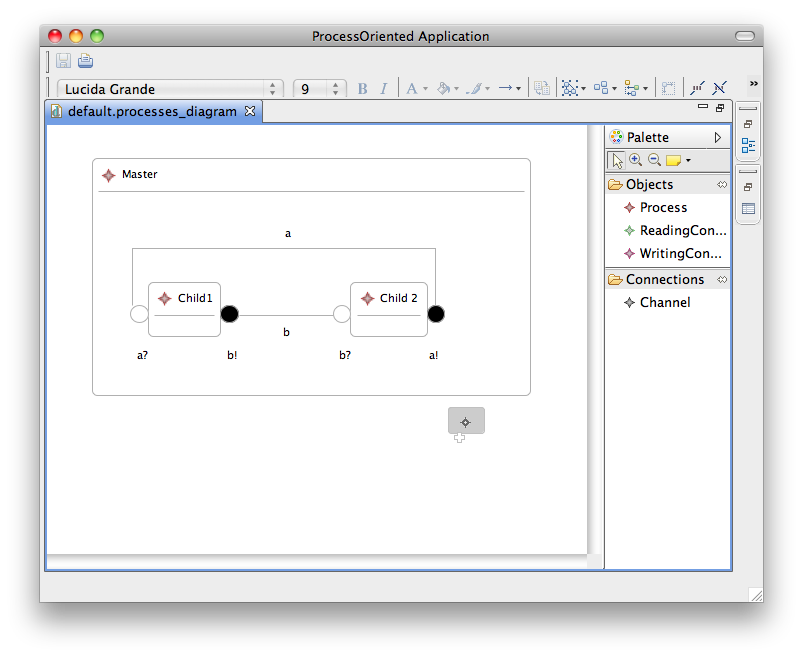
\includegraphics[width=12.75cm]{6.Evaluation/images/user_driven/po_final_editor.png}
	\caption{Final version of the prototypical graphical model editor.}
	\label{fig:po_final_graphical_editor}
\end{figure}

The graphical model editor was implemented using EMF. The metamodel was specified in Ecore, the metamodelling language of EMF, and the graphical editor was generated from the metamodel using GMF. Section~\ref{sec:mde_tools} describes in more detail the way in which EMF and GMF can be used to specify metamodels and to generate graphical model editors.

The process-oriented metamodel was developed iteratively, and the six iterations are described in Appendix~\ref{ProcessOriented}. During each iteration, the metamodel was changed. The evaluation described here uses an example of metamodel changes from the fifth iteration of the project. The way in which development proceeded during that iteration is described in Section~\ref{sec:po_it5} and summarised below.

\subsubsection{Aim of Iteration 5}
Iteration 5 of the process-oriented example was used to describe Epsilon Flock in \ref{subsec:flock_examples}. The purpose of the iteration was to refine the way in which connection points were represented. At the start of the iteration, the graphical model editor could be used to draw processes, channels and connection points. However, no distinction was made between reading and writing connection points.

Figure~\ref{fig:po_original_editor} shows a model represented in the graphical model editor before the iteration began. The model contains two processes (depicted as boxes), \texttt{P1} and \texttt{P2}, one channel (depicted as a line), \texttt{a}, and two connection points (depicted as circles), \texttt{a!} and \texttt{a?}.

\begin{figure}[htbp]
	\centering
	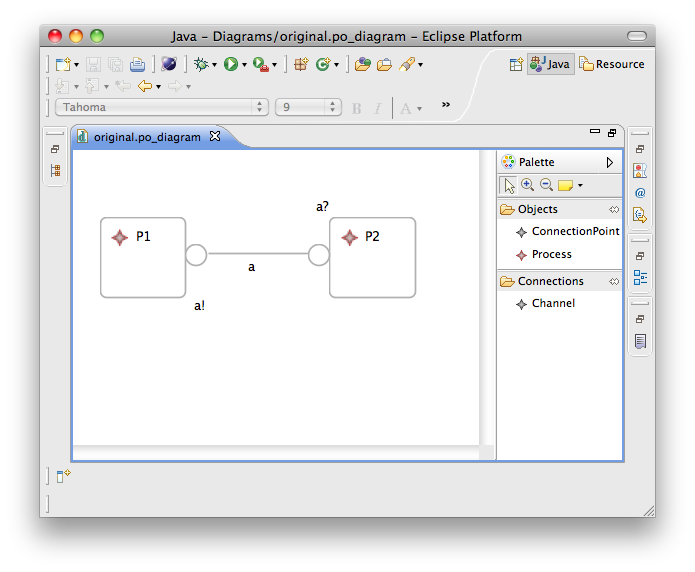
\includegraphics[width=12.75cm]{6.Evaluation/images/user_driven/po_original_editor.png}
	\caption{The graphical editor at the start of the iteration.}
	\label{fig:po_original_editor}
\end{figure}


The aim of the iteration was to distinguish between reading and writing connection points in the graphical notation. The former are used to receive messages, and the latter to send messages. In Figure~\ref{fig:po_original_editor}, \texttt{a?} is intended to represent a reading connection point, and \texttt{a!} a writing connection point. Sampson and I decided that the editor should be changed so that black circles would be used to represent writing connection points, and white circles to represent reading connection points. At the end of the iteration the model shown in Figure~\ref{fig:po_original_editor} would be represented as shown in Figure~\ref{fig:po_evolved_editor}. Furthermore, the editor would ensure that \texttt{a?} was used only as the reader of a channel, and \texttt{a!} only as the writer of a channel. Before the iteration started, the editor did not enforce this constraint.

\begin{figure}[htbp]
	\centering
	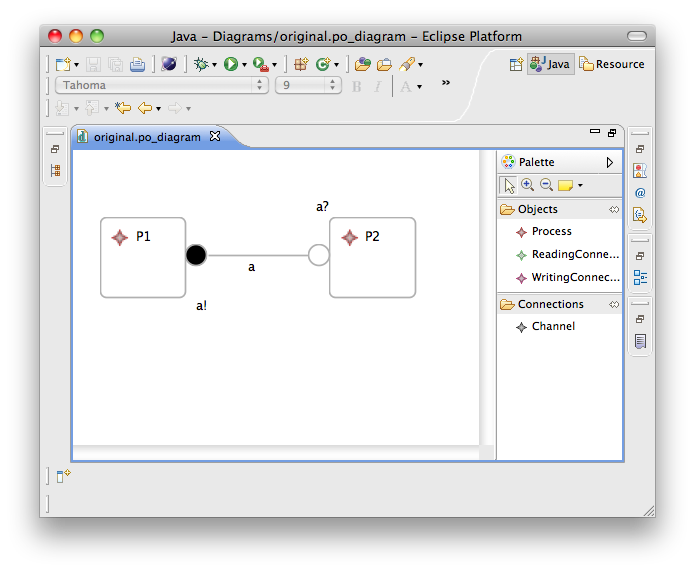
\includegraphics[width=12.75cm]{6.Evaluation/images/user_driven/po_evolved_editor.png}
	\caption{The graphical editor at the end of the iteration.}
	\label{fig:po_evolved_editor}
\end{figure}


\subsubsection{Metamodel changes during Iteration 5}
Before the iteration started, the metamodel, shown in Figure~\ref{fig:po_original_mm}, did not distinguish between reading and writing \texttt{Co\-nn\-ec\-ti\-o\-nPo\-i\-nt}s. A \texttt{Co\-nn\-ec\-ti\-o\-nPo\-i\-nt} could be associated with a \texttt{Ch\-an\-nel} via the \texttt{re\-ad\-er} or \texttt{wr\-it\-er} reference of \texttt{Ch\-an\-nel}, but the type of a \texttt{Co\-nn\-ec\-ti\-o\-nPo\-i\-nt} was not specified explicitly.

The way in which connection points were modelled was changed, resulting in the metaclasses shown in Figure~\ref{fig:po_evolved_mm}. \texttt{Co\-nn\-ec\-ti\-o\-nPo\-i\-nt} was made abstract, and two subtypes, \texttt{Re\-ad\-i\-ngCo\-nn\-ec\-ti\-o\-nPo\-i\-nt} and \texttt{Wr\-i\-ti\-ngCo\-nn\-ec\-ti\-o\-nPo\-i\-nt}, were introduced. The \texttt{re\-ad\-er} and \texttt{wr\-it\-er} references of \texttt{Ch\-an\-n\-el} were changed to refer to the new subtypes. The evolved metamodel correctly prevented the use of a \texttt{Co\-nn\-ec\-ti\-o\-nPo\-i\-nt} as both a \texttt{re\-ad\-er} and a \texttt{wr\-it\-er}.

\begin{figure}[htbp]
	\centering
	\subfigure[Part of the original metamodel.]
	{
	    \label{fig:po_original_mm}
	    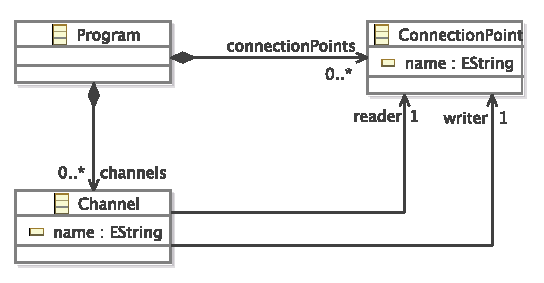
\includegraphics[width=7.5cm]{6.Evaluation/images/user_driven/po_before.pdf}
	}
	\subfigure[Part of the evolved metamodel.]
	{
	    \label{fig:po_evolved_mm}
	    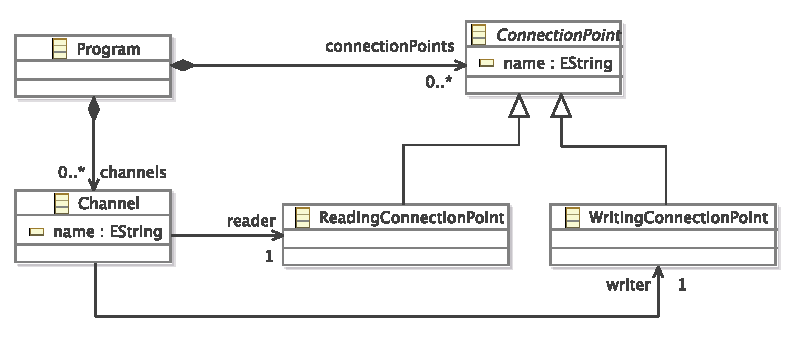
\includegraphics[width=11cm]{6.Evaluation/images/user_driven/po_after.pdf}
	}
	\caption{Process-oriented metamodel evolution.}
\label{fig:po_mms}
\end{figure}

Following the metamodel changes, a new version of the graphical editor was generated automatically from the metamodel using GMF. An annotation -- not shown in Figure~\ref{fig:po_evolved_mm} -- on the \texttt{Wr\-i\-ti\-ngCo\-nn\-ec\-ti\-o\-nPo\-i\-nt} class was used to indicate to GMF that black circles were to be used to represent writing connection points in the graphical notation.

\subsubsection{Testing during Iteration 5}
Testing the new version of the graphical editor highlighted the need for model migration. Attempting to load existing models, such as the one shown in Figure~\ref{fig:po_original_editor}, caused an error because \texttt{Co\-nn\-ec\-ti\-onP\-oi\-nt} was now an abstract class. Any model specifying at least one connection point no longer conformed to the metamodel. Model migration was performed to re-establish conformance and to allow the models to be loaded. 

Several models, presented in Appendix~\ref{ProcessOriented}, had been constructed when testing previous versions of the graphical editor. The models were used during each iteration to ensure that any changes had not introduced regressions. After the metamodel changes described above, the test models could no longer be loaded and required migration. A developer-driven co-evolution approach was not suitable for the development of process-oriented editor because only a few small models required migration in each iteration. A user-driven co-evolution approach was used instead, but, as no structures dedicated to user-driven co-evolution were available, co-evolution was performed by manually editing the storage representation of models. 

The sequel describes the way in which migration was performed during the development of the process-oriented metamodel, without dedicated structures for performing user-driven co-evolution. Section~\ref{subsec:user-driven_co-evolution_with_dedicated_structures} describes the way in which migration could have been performed using two of the structures presented in Chapter~\ref{Implementation}. The section concludes by comparing the two approaches.

\subsection{User-Driven Co-Evolution with EMF}
\label{subsec:user-driven_co-evolution_with_emf}
During the development of the process-oriented metamodel, no dedicated structures for performing user-driven co-evolution were available. Instead, migration was performed using only those tools available in EMF, as described below.

Migration with EMF involved identifying and fixing conformance errors, using the workflow shown in Figure~\ref{fig:emf_process}. The workflow was first discussed in Chapter~\ref{Analysis}. When the user attempts to load a model, EMF automatically checks the conformance of the model. If the model does not conform to its metamodel, loading fails. To re-establish conformance, the user must edit by hand the underlying storage representation of the model, XMI. Recall that co-evolution is an iterative process because EMF uses a multi-pass XMI parser and cannot report all categories of conformance problem in the first pass.

One of the test models, shown in Figure~\ref{fig:po_original_editor}, is now used to illustrate the way in which user-driven co-evolution was performed using the workflow shown in Figure~\ref{fig:emf_process}. For the test model shown in Figure~\ref{fig:po_original_editor}, the conformance problems shown in the bottom pane (and by the error markers in the left-hand margin of the top pane) of Figure~\ref{fig:po_original_xmi} were reported by EMF. For example, the first conformance problem reported is shown in the tooltip in Figure~\ref{fig:po_original_xmi}, and states that a \texttt{ClassNotFoundException} was encountered because the ``Class `ConnectionPoint' is not found or is abstract.''

\begin{figure}[htbp]
	\centering
		\includegraphics*[viewport=80 280 600 550,height=5.75cm]{6.Evaluation/images/user_driven/emf_process.pdf}
	\caption{User-driven co-evolution with EMF}
	\label{fig:emf_process}
\end{figure}

\begin{figure}[htbp]
	\centering
	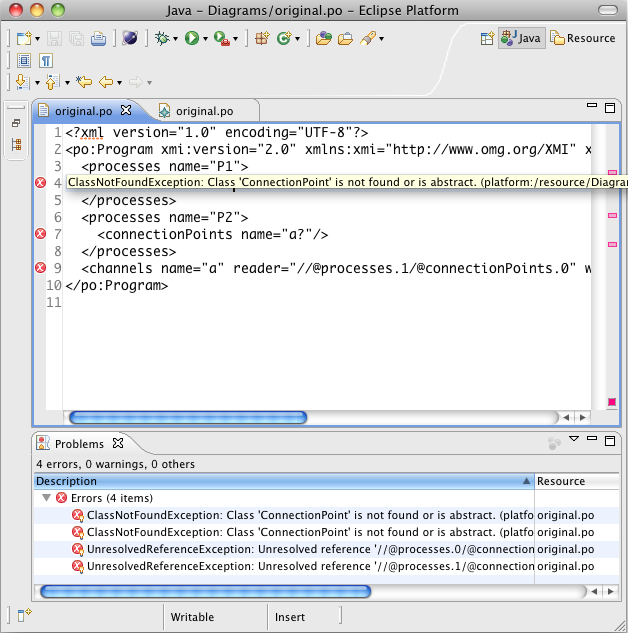
\includegraphics[width=12.75cm]{6.Evaluation/images/user_driven/po_original_xmi.png}
	\caption{XMI prior to migration}
	\label{fig:po_original_xmi}
\end{figure}

The conformance problems were fixed by editing the XMI shown in Figure~\ref{fig:po_original_xmi}, producing the XMI shown in Figure~\ref{fig:po_migrated_xmi}. The type of each connection point element was changed to either \texttt{Re\-ad\-i\-ngCo\-nn\-ec\-ti\-o\-nPo\-i\-nt} or \texttt{Wr\-i\-ti\-ngCo\-nn\-ec\-ti\-o\-nPo\-i\-nt}. The former was used when the connection point was referenced via the \texttt{reader} reference of \texttt{Channel}, and the latter otherwise. The reconciled XMI is shown in Figure~\ref{fig:po_migrated_xmi}. On lines 4 and 7, the connection point model elements have been changed to include \texttt{xsi:type} attributes, which specify whether the connection point should instantiate \texttt{Re\-ad\-i\-ngCo\-nn\-ec\-ti\-o\-nPo\-i\-nt} or \texttt{Wr\-i\-ti\-ngCo\-nn\-ec\-ti\-o\-nPo\-i\-nt}.

\begin{figure}[htbp]
	\centering
	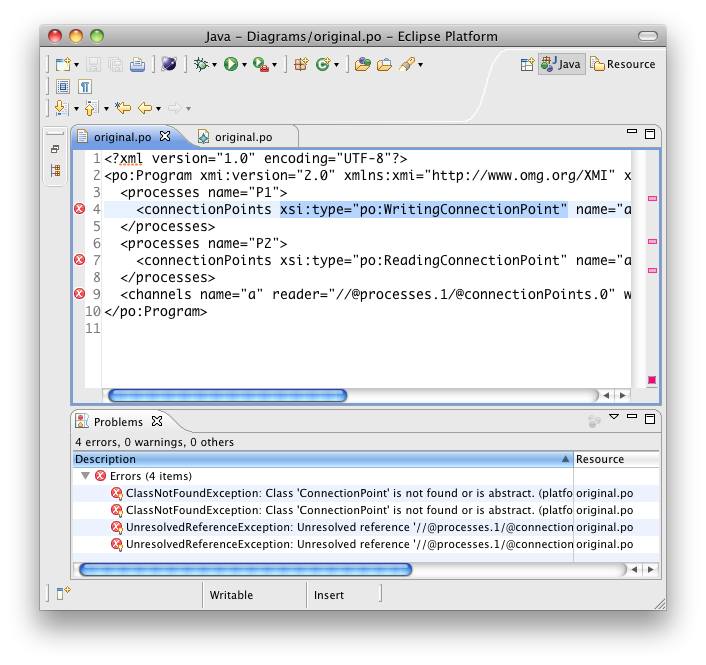
\includegraphics[width=12.75cm]{6.Evaluation/images/user_driven/po_migrated_xmi.png}
	\caption{XMI after migration}
	\label{fig:po_migrated_xmi}
\end{figure}

Reconciling the conformance problems by editing the XMI required considerable knowledge of the XMI specification. For example, the \texttt{xsi:type} attribute is used to specify the type of the connection point model elements. In fact, it must be included for those model elements. However, for the other model elements in Figure~\ref{fig:po_migrated_xmi} the \texttt{xsi:type} attribute is not necessary, and is omitted. When and how to use the \texttt{xsi:type} attribute is discussed further in the sidebar, in the XMI specification \cite{xmi}, and by the developers of EMF \cite{steinberg09emf}. EMF abstracts away from XMI, and typically users do not interact directly with XMI. Therefore, it may be reasonable to assume that EMF users might not be familiar with XMI, and implementation details such as the \texttt{xsi:type} attribute.

\begin{figure*}[tbp]
	\begin{framed}
	\textbf{The \texttt{xsi:type} attribute} \\
	In XMI, each model element must indicate the metaclass that it instantiates. Typically, the \texttt{xsi:type} attribute is used for this purpose. For example, the model element on line 4 of Figure~\ref{fig:po_migrated_xmi} instantiates the metaclass named \texttt{Wr\-i\-ti\-ngCo\-nn\-ec\-ti\-o\-nPo\-i\-nt}. To reduce the size of models on disk, the XMI specification allows type information to be omitted when it can be inferred. For example, line 9 of Figure~\ref{fig:po_migrated_xmi} defines a model element that is contained in the \texttt{ch\-an\-ne\-ls} reference of a \texttt{Pr\-o\-ce\-ss}. Because the \texttt{ch\-an\-ne\-ls} reference can contain only one type of model element (\texttt{Ch\-an\-n\-el}), the \texttt{xsi:type} attribute can be omitted, and the type information is inferred from the metamodel.
	\end{framed}
\end{figure*}

% For every instance of \texttt{Ch\-an\-n\-el} that referenced a \texttt{Co\-nn\-ec\-ti\-o\-nPo\-i\-nt}, the following message was produced: ``Unresolved reference `\texttt{<ID>}' '' where \texttt{<ID>} was the identifier of the referenced \texttt{Co\-nn\-ec\-ti\-o\-nPo\-i\-nt}.

% Notice that conformance problem markers are still present in Figure~\ref{fig:po_original_editor}

During the development of the process-oriented editor, some mistakes were made when the XMI of the test models was edited by hand. For example, the wrong subtype of \texttt{Co\-nn\-ec\-ti\-onPo\-in\-t} was used as the type of several connection point model elements. The mistake occurred because XMI identifies model elements using an offset from the root of the document. For example, consider the XMI shown in Figure~\ref{fig:po_migrated_xmi}. The channel on line 9 specifies the value ``//@processes.1/@connectionPoints.0'' for its \texttt{re\-ad\-er} attribute. The value is an XMI path referencing the first connection point (``@connectionPoints.0'') contained in the second process (``@processes.1'') of this document (``//''); in other words the connection point on line 7. One of Sampson's models contained many channels and connection points and incorrectly counting the connection points in the model led to several mistakes during the manual editing of the XMI. Each time a mistake was made when reconciling the XMI by hand, another loop around the workflow shown in Figure~\ref{fig:emf_process} was required.

As demonstrated above, migration using only the tools provided by EMF can be iterative and error-prone. The sequel demonstrates that, by using the dedicated structures described in Chapter~\ref{Implementation}, migration can be performed in one iteration, without requiring the developer to switch between conformance reporting and model migration tools. In addition, the sequel suggests how the mistake described above might be avoided by using Epsilon HUTN rather than XMI for manually migrating models.

\subsection{User-Driven Co-Evolution with Dedicated Structures}
\label{subsec:user-driven_co-evolution_with_dedicated_structures}

Chapter~\ref{Implementation} describes two structures that can be used to perform user-driven co-evolution. Here, the functionality of the two structures, a metamodel-independent syntax and a textual modelling notation, is summarised. Subsequently, an approach that uses the metamodel-independent syntax and the textual modelling notation for migrating the model from the process-oriented example is presented. The model migration example presented in this section was performed retrospectively by the author after the process-oriented editor was completed, and demonstrates how migration might have been achieved with dedicated structures for user-driven co-evolution. The sequel compares the user-driven co-evolution approach presented in this section with the approach presented in Section~\ref{subsec:user-driven_co-evolution_with_emf}.

The metamodel-independent syntax presented in Section~\ref{sec:mmi_syntax} allows non-conformant models to be loaded with EMF, and for the conformance of models to be checked against any metamodel. Epsilon HUTN, the textual modelling notation presented in Section~\ref{sec:notation} is underpinned by \changed{``built atop'' changed to ``underpinned by''} the metamodel-independent syntax and is an alternative to XMI for representing models in a textual format. Together, the two structures can be used for performing user-driven co-evolution using the workflow shown in Figure~\ref{fig:hutn_process}. The workflow was first discussed in Chapter~\ref{Implementation}. First, the user attempts to load a model in the graphical editor. If the model is non-conformant and cannot be loaded, the user clicks the ``Generate HUTN'' menu item, and the model is loaded with the metamodel-independent syntax and then a HUTN representation of the model is generated by Epsilon HUTN. The generated HUTN is presented in an editor that automatically reports conformance problems using the metamodel-independent syntax. The user edits the HUTN to reconcile conformance problems, and the conformance report is automatically updated as the user edits the model. When the conformance problems are fixed, XMI for the conformant model is automatically generated, and migration is complete. The model can then be loaded in the graphical editor.

\begin{figure}[htbp]
	\centering
	\includegraphics*[viewport=80 290 760 550,height=4.75cm]{6.Evaluation/images/user_driven/hutn_process.pdf}
	\caption{User-driven co-evolution with dedicated structures}
	\label{fig:hutn_process}
\end{figure}

The way in which the workflow shown in Figure~\ref{fig:hutn_process} was used to perform user-driven co-evolution for the process-oriented metamodel is now demonstrated. For the model shown in Figure~\ref{fig:po_original_editor}, the HUTN shown in Figure~\ref{fig:po_hutn} was generated by invoking the automatic XMI-to-HUTN transformation. The HUTN development tools automatically present any conformance problems, as shown in the bottom pane (and the left-hand margin of the top pane) in Figure~\ref{fig:po_hutn}.

\begin{figure}[htbp]
  \centering
  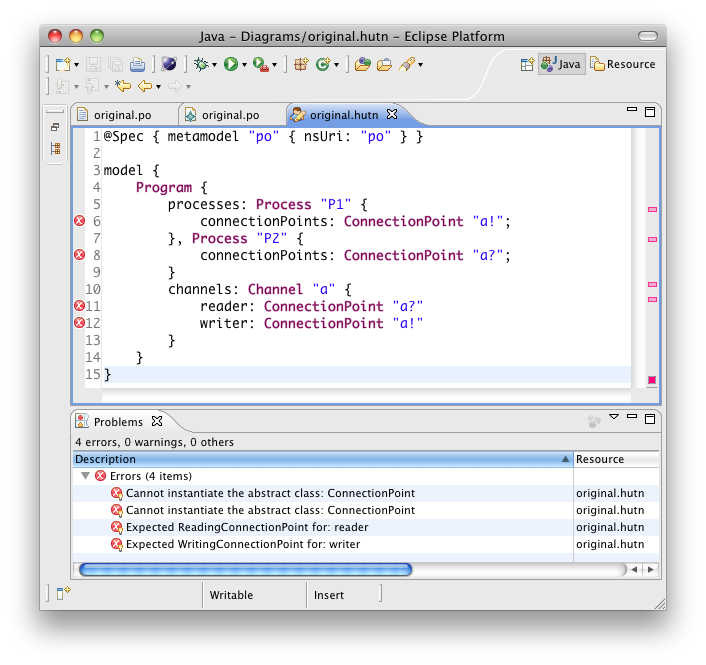
\includegraphics[width=12.75cm]{6.Evaluation/images/user_driven/po_hutn.png}
  \caption{HUTN source prior to migration}
  \label{fig:po_hutn}
\end{figure}

Conformance problems are reconciled manually by the user, who edits the HUTN source. Conformance is automatically checked whenever the HUTN is changed. For example, Figure~\ref{fig:po_hutn_partial} shows the HUTN editor when migration is partially complete. Some of the conformance problems have been reconciled, and the associated error-markers are no longer displayed in the left-hand margin.

\begin{figure}[htbp]
  \centering
  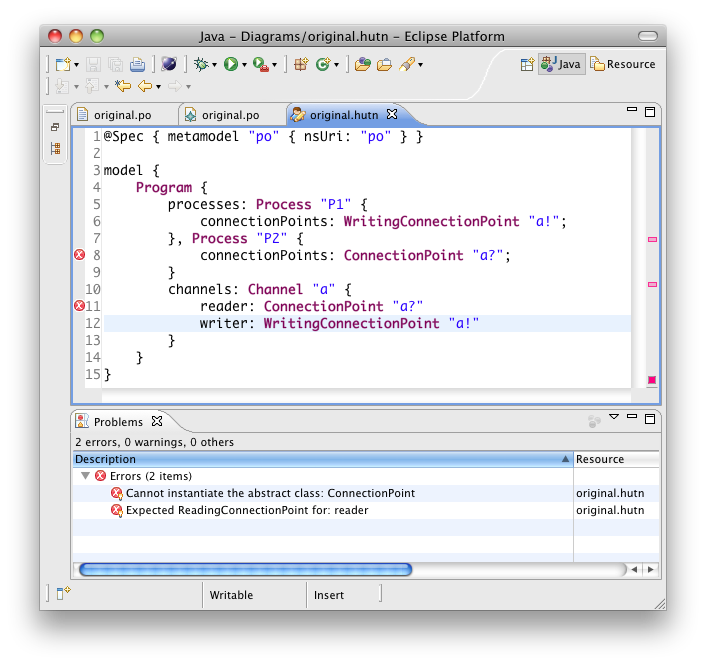
\includegraphics[width=12.75cm]{6.Evaluation/images/user_driven/po_hutn_partial.png}
  \caption{HUTN source part way through migration}
  \label{fig:po_hutn_partial}
\end{figure}

When no conformance errors remain, Epsilon HUTN automatically generates XMI for reconciled model, and the user can now successfully load the migrated model with the graphical editor.

\subsection{Comparison}
\label{subsec:user_driven_example_comparison}
To suggest ways in which dedicated structures for user-driven co-evolution might increase developer productivity, the two user-driven co-evolution approaches demonstrated above are now compared. The first approach, described in Section~\ref{subsec:user-driven_co-evolution_with_emf}, uses only those tools available in EMF for performing user-driven co-evolution, while the second approach, described in Section~\ref{subsec:user-driven_co-evolution_with_dedicated_structures} uses two of the structures introduced in Chapter~\ref{Implementation}. Applying the approaches to the process-oriented example highlighted differences between the modelling notations used, and the way in which conformance problems were reported.

\subsubsection{Differences in modelling notation}
For reconciling conformance problems, the two approaches used different modelling notations, XMI and Epsilon HUTN. Differences in notation that might influence developer productivity during user-driven co-evolution are now discussed. However, further work is required to more rigorously explore the extent to which developer productivity is affected by the modelling notation, as discussed in Section~\ref{subsec:user_driven_further_work}.

The way in which the type of a model element is specified is different in XMI and HUTN. In XMI, type information can be omitted in some circumstances, but must be included in others. In HUTN, type information is mandatory for every model element. Consequently, every HUTN document contains examples of how type information should be specified, whereas XMI documents may not. 

Reference values use paths in XMI (such as \texttt{//@pro\-ces\-ses.1/@con\-nec\-ti\-onPo\-in\-ts.0}) and names (such as \texttt{a?}) in HUTN. XMI paths are constructed in terms of a document's structure and, as such, rely on implementation details. The name of a model element, on the other hand, is specified in the model, and does not rely on any implementation details. Consequently, it is conceivable that fewer mistakes will be made during user-driven co-evolution when reference values are specified by name rather than with the structural details of a model.

\subsubsection{Differences in conformance reports}
The two approaches differ in the way in which conformance problems were reported, and, as a consequence, the first approach was iterative and the second was not. The differences might influence developer productivity during user-driven co-evolution. Again, further work is required to rigorously explore the extent to which developer productivity is affected by the differences in conformance reporting, as discussed in Section~\ref{subsec:user_driven_further_work}.

With EMF, user-driven co-evolution is an iterative process. Conformance errors are fixed by the user, who then reloads the reconciled model (with, for example, a graphical editor). Each time the model is loaded, further conformance problems might be reported when, for example, the user makes a mistake when reconciling the model. By contrast, the implementation of HUTN described in Section~\ref{sec:notation} uses a background compiler that checks conformance while the user edits the HUTN source. When the user makes a mistake reconciling the HUTN source, the error is reported immediately, and does not require the model to be loaded in the graphical editor.

Although not demonstrated here, user-driven co-evolution would, for some types of metamodel changes, remain an iterative process even if EMF performed conformance checking in the background. Because EMF uses a multi-pass parser, some types of conformance problem are reported before other types. For example, conformance problems relating to multiplicity constraints (e.g. a process does not specify a name, but name is a mandatory attribute) are reported after all other types of conformance problem. When several types of conformance problem have been affected by metamodel changes, user-driven co-evolution with EMF would remain an iterative process. Single-pass, background parsing is required to display all conformance problems while the user migrates a model.

\subsection{Towards a more thorough comparison}
\label{subsec:user_driven_further_work}
Extensions to the evaluation of user-driven co-evolution are now discussed. In particular, alternative comparison methods might enable a more rigorous exploration of the ways in which dedicated structures for performing user-driven co-evolution influence developer productivity.

A comprehensive user study, involving hundreds of users, is one means for exploring the extent to which productivity varies when dedicated structures are used to perform user-driven co-evolution. Ideally, participants for the study would constitute a large and representative sample of the users of EMF. Productivity might be measured by the time taken to perform co-evolution. To remove a potential source of bias, several examples of co-evolution might be used.

% Autocompletion
% Iterative problem reporting might be good - perhaps it could be used to show "likely" root cause problems first, and problems less likely to be a root cause later?s
% Other types of XMI ID: UUID, derived


Locating a reasonable number of participants and co-evolution examples for a comprehensive user study was not feasible in the context of this thesis. Nevertheless, the comparison presented in Section~\ref{subsec:user_driven_example_comparison} suggests that productivity might be increased when using dedicated structures for user-driven co-evolution. By demonstrating an approach to user-driven co-evolution that uses dedicated structures, this thesis provides a foundation for further, more rigorous evaluation. For example, the HUTN specification \cite{hutn} makes claims about the human-usability of the notation, but the usability of HUTN has not been studied or compared with other modelling notations. Epsilon HUTN (Section~\ref{sec:notation}) is a reference implementation of HUTN and, as demonstrated by the evaluation presented here, facilitates the evaluation of HUTN and the comparison of HUTN to other modelling notations, such as XMI.


\subsection{Summary}
\label{subsec:user_driven_example_summary}
This section has demonstrated two approaches to user-driven co-evolution using a co-evolution example from a project in which a graphical model editor was created for process-oriented programs. The first approach used the structures available in EMF alone, while the second approach used two of the structures described in Chapter~\ref{Implementation}. Comparing the two approaches highlighted differences between the way in which conformance problems were reported and between the modelling notations used to reconcile conformance problems. The comparison described in Section~\ref{subsec:user_driven_example_comparison} suggests that developer productivity might be increased by using the second approach, but, as discussed in Section~\ref{subsec:user_driven_further_work}, further work is required to more rigorously evaluate this claim.

